\documentclass[12pt, french]{article}

\usepackage{fancyhdr, fancybox, lastpage}
\usepackage[most]{tcolorbox}
\usepackage[a4paper, margin={0.3in, .75in}]{geometry}
\usepackage{wrapfig}
\pagestyle{fancy}
\renewcommand\headrulewidth{1pt}
\renewcommand\footrulewidth{1pt}
\fancyhf{}
\rhead{ \em{Zakaria Haouzan}}
\lhead[C]{\em{2ème année baccalauréat Sciences Physiques}}
\chead[C]{}
\rfoot[C]{}
\lfoot[R]{}
\cfoot[]{\em{Page \thepage / \pageref{LastPage}}}


\newtcolorbox{Box2}[2][]{
                lower separated=false,
                colback=white,
colframe=white!20!black,fonttitle=\bfseries,
colbacktitle=white!30!gray,
coltitle=black,
enhanced,
attach boxed title to top left={yshift=-0.1in,xshift=0.15in},
title=#2,#1}


\begin{document}
\begin{center}
   \shadowbox {\bf{Dipôle RC }}
\end{center}

\vspace{-0.2cm}
%\begin{wrapfigure}{r}{0.22\textwidth}
  %\begin{center}
	  %\vspace{-0.6cm}
	%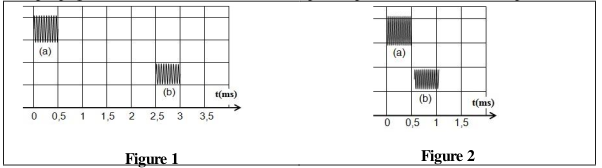
\includegraphics[width=0.22\textwidth]{./img/Ex2.png}
  %\end{center}
%\end{wrapfigure}



%%_________________________Exercice ! :"_________________________Exercice
   \begin{Box2}{Exercice 1 :}
	   \begin{wrapfigure}[5]{r}{0.46\textwidth}
  \begin{center}
	  \vspace{-0.6cm}
	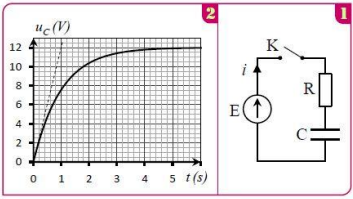
\includegraphics[width=0.46\textwidth]{./img/ex00_charge.png}
  \end{center}
\end{wrapfigure}


Pour déterminer la capacité d’un condensateur on réalise le montage de la figure 1 qui est
formé des éléments suivants :
\begin{itemize}
	\item un générateur idéal de tension de force électromotrice $E=12V$.
	\item un conducteur ohmique de résistance $R=1K\Omega$.
	\item un condensateur déchargé de capacité C et un interrupteur K et des fils de connexion .
\end{itemize}
A l’instant t=0 on ferme l’interrupteur K et on suit par un dispositif convenable les variations de la tension
appliquée aux bornes du condensateur en fonction du temps et on obtient la figure 2.

\textbf{1. }représenter sur la figure 1 dans la convention récepteur les tensions $u_C$ et $u_R$.

\textbf{2. }montrer que l’équation différentielle vérifié par la tension aux bornes du condensateur est : $RC.\frac{du_C}{dt}$+$u_C$=$E$.

\textbf{3. }Trouver les expressions de $A$ et $\tau$ pour que l’expression $u_C = A(1-e^{-\frac{t}{\tau}} )$ soit solution de l’équation différentielle.

\textbf{4. }Par l’analyse dimensionnelle montrer que $\tau$ a une dimension du temps.

\textbf{5. }trouver $\tau$ graphiquement et montrer que $C=1mF$.

\textbf{6. }Calculer l’énergie électrique $E_e$ stockée dans le condensateur dans le régime permanent.
   \end{Box2}


%%_________________________Exercice !2 :"_________________________Exercice


   \begin{Box2}{Exercice 2 : }
	   Pour étudier la charge du
condensateur, le professeur réalise le
montage de la figure (1) constitué des
éléments suivants :
\\- Un générateur idéal de courant
qui alimente le circuit par un
courant électrique d'intensité
constante $I_0 = 2.10^{-5}A$.
\\-Un conducteur ohmique de résistance $R_0$.
\\- Un condensateur de capacité C;
\\- Un interrupteur K.
\\À $t_0 =0$, le professeur ferme l'interrupteur K et suit à l'aide d'un dispositif convenable, les variations
de la tension $u_C(t)$ aux bornes du condensateur. La figure (2) représente la courbe obtenue.
\\\textbf{1. }En exploitant la courbe, déterminer l'expression de la tension $u_C(t)$.
\\\textbf{2. }Montrer que $C=1\mu.F$
  
\begin{center}
	  %\vspace{-0.6cm}
	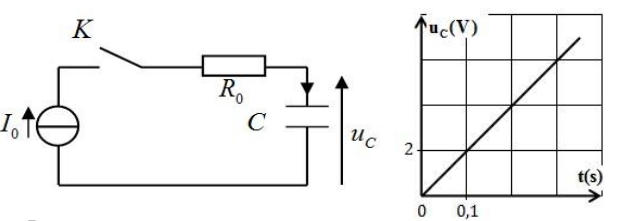
\includegraphics[width=0.6\textwidth]{./img/ex_02.png}
	%\captiocc{}
  \end{center}




   \end{Box2}
\begin{Box2}{Exercice 3 :  }
\begin{wrapfigure}{r}{0.16\textwidth}
  \begin{center}
	  \vspace{-0.6cm}
	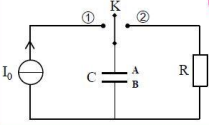
\includegraphics[width=0.16\textwidth]{./img/ex_02_circuit.png}
	\caption{}
  \end{center}
\end{wrapfigure}

On réalise le montage de la figure1 formé de :
\begin{itemize}
	\item un générateur idéal du courant qui alimente le circuit par un courant d’intensité .
	\item un condensateur de capacité C initialement déchargé.
	\item un conducteur ohmique de résistance R.
	\item un interrupteur K a deux positions 1 et 2.
\end{itemize}

\begin{wrapfigure}{r}{0.26\textwidth}
  \begin{center}
	  \vspace{-5cm}
	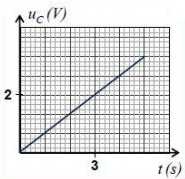
\includegraphics[width=0.26\textwidth]{./img/ex_02_fig2.jpg}
	\caption{}
	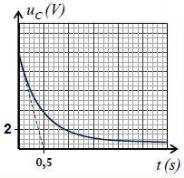
\includegraphics[width=0.26\textwidth]{./img/ex_02_fig3.jpg}
	\caption{}
  \end{center}
\end{wrapfigure}



\textbf{I- }A $t=0$ on bascule l’interrupteur à la position 1 et on suit les variations \\de la tension $u_C$ en fonction du temps et on obtient la courbe de la figure 2.

\textbf{1. }Déterminer l’armature négative.

\textbf{2. }Montrer que l’expression de la tension aux bornes du
condensateur s’écrit : $u_C = \frac{I_0}{C}.t$

\textbf{3. }Vérifie que : $C =1,5.10^{-3}F $

\textbf{4. }Calculer l’énergie $E_e$ électrique stockée dans le condensateur à $t= 3s$.

\textbf{II. }Lorsque la tension aux bornes du condensateur est égale à 10V on bascule l’interrupteur à la position 2 et on obtient la courbe de la figure 3.

\textbf{5. }Déterminer l’équation différentielle vérifié par $u_C$ .

\textbf{6. }La solution de l’équation différentielle s’écrit : $u_C = A.e^{-\alpha.t}$.déterminer les expressions de $A$ et $\alpha$ en fonctions des paramètres du circuit.

\textbf{7. }Déterminer la valeur de $\tau$ et déduire la valeur de la résistance R.

\textbf{8. }Montrer que l’expression de l’intensité du courant est : $i = -0,03.e^{-2t}$

\textbf{9. }Expliquer comment on peut choisir la valeur de R pour avoir une décharge rapide.
\end{Box2}

%%_________________________Exercice ! 3:"_________________________Exercice
\begin{Box2}{Exercice 4 : }

	\begin{wrapfigure}{r}{0.26\textwidth}
  \begin{center}
	  \vspace{-0.8cm}
	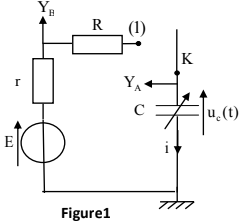
\includegraphics[width=0.26\textwidth]{./img/ex04_1.png}
	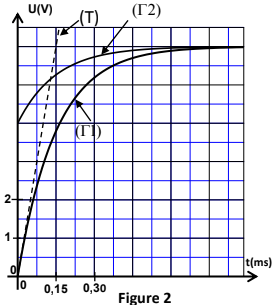
\includegraphics[width=0.26\textwidth]{./img/ex04_2.png}
	\caption{}
  \end{center}
\end{wrapfigure}




	L’objectif de cet exercice est d’étudier la réponse d’un dipôle RC  à un échelon de tension .On réalise le circuit électrique schématisé sur la figure 1.Ce circuit comporte : 
\\Un générateur de f.e.m. E et de résistance
interne négligeable ;
\\- Deux conducteurs ohmiques de résistance r
et $R=20\Omega$;
\\- Un condensateur de capacité C réglable,
initialement déchargé ;
\\- Un interrupteur K .

On fixe la capacité du condensateur sur la valeur $C_0$. A un instant de date $t=0$ , on place l’interrupteur
K en position (1) .Un système d’acquisition informatisé permet de tracer les courbes $(\Gamma 1)$ et$(\Gamma 2)$ de la
figure 2 représentant les tensions obtenues en utilisant les voies $Y_A$ et $Y_B$
(fig.1) .La droite (T) représente la tangente à la courbe $(\Gamma 1)$ à t=0.

\textbf{1. }Identifier parmi les courbes $(\Gamma 1)$ et $(\Gamma 2)$ celle qui représente la tension $u_C(t)$.

\textbf{2. }Etablir l’équation différentielle vérifiée par la tension $u_C(t)$.

\textbf{3. }Montrer que l’expression de l’intensité du courant juste après avoir placé l’interrupteur en position (1) est : $i_0 = \frac{E}{R+r}$

\textbf{4. }A l’aide des deux courbes : Déterminer la valeur de r et Montrer que $C_0 = 5\mu.F$  

\end{Box2}

%%_________________________Exercice 4 : _________________________Exercice
%\begin{Box2}{Exercice 4 :corde élastique }
%4
%\end{Box2}
%%\vspace{2cm}
%\begin{center}
   %\Large{ \em{Exercices Supplémentaires}}
%\end{center}


%\vspace{-0.7cm}
%%%_________________________Exercice 5 : _________________________Exercice
%\begin{Box2}{Exercice 5 :Les ondes sonores }

%\end{Box2}
%%%_________________________Exercice 6 : _________________________Exercice
%\begin{Box2}{Exercice 6 : échographie}

%\end{Box2}

\end{document}
